%--------------------------------------------------------------------------------------------------
\section{Image Recognition Models}
\label{rel:sec_imrecon}
Image recognition is a substask of computer science that aims at replicating human vision capabilities 
with a machine. Arguably, it is with the improvement and interaction of the three fundamental tasks 
of computer vision (Recognition, Reconstruction and Reorganization) \autocite{malik2016three} that we 
find this field moves forward. Interestingly, improvements in one these fundamental Rs can be 
used to drive forth its peers; moreover, (words).




%1960s, first thesis, image processing, pattern recognition
%1970s foundational work on image recognition
%1980 vision applied to maths, geometry, control theory, optimization
%1990s geometric analysis coplete, graphics,statistical learning
%200s advances in visual recognition, practical applications

Ultimately, it was with inspiration on studies on neuroscience \autocite{hubel1959receptive} that the 
development of \glspl{nn} started. In particular, the Neocognitron \autocite{fukushima1975cognitron} 
proposes the first \gls{nn} where kernel operations, feature aggregation in a hierarchical 
manner and non-linearities stand out as these contributions can be seen as the main components of a 
most recent image recogniton models.

Still, the Neocognitron's hierarchical properties and aggregation didn't really achieve 
a great deal of momentum on early days; around this time, other image recognition models were being 
used yielding better results, examples of this can be seen with the amount of traditional machine 
learning based methods that dominated this task around that time. Still getting close to the dawn 
of the 1990s, Yann LeCunn proposed LeNet to perform digit recognition \autocite{lecun1998gradient}.\\

\subsection{Convolutional Neural Networks}
\label{rel:sub_cnn}
Starting with LeNet, the convolution took prominence as the fundamental building block 
of most current image recognition models. On itself, a convolutional layer operates by the 
interaction of a kernel with a set of features at any given layer. This interaction depends in 
direct correlation with the kernel size, mediated by its width and height. Furthermore, 
these kernels are meant to project features into different spaces; with this in mind we point out 
that convolutions are mostly a local operation. 
%Figure \ref{fig:conv_local} illustrates these 
%properties of the convolution operation.
%\begin{figure}[h]
    \centering
    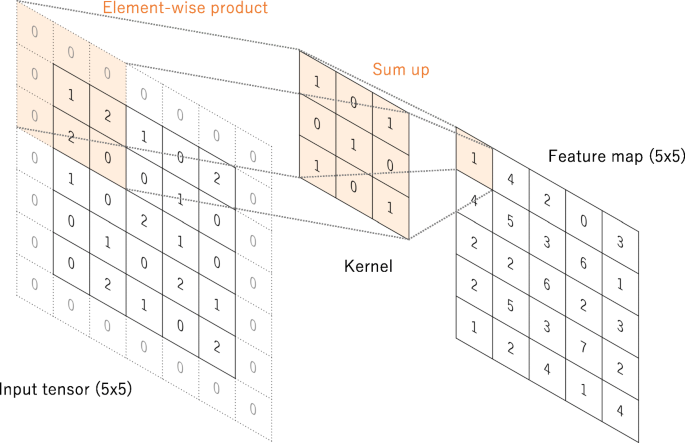
\includegraphics[width=\textwidth]{fig/rel/images/conv_not_proper.png}
    \caption{Illustration of the convolution operation. Properties, parameters and behaviour.}
    \label{fig:conv_local}
\end{figure}

\noindent On top of convolutions, LeNet led to the introduction of more components of \glspl{cnn}: 
pooling operations and non-linearities. Pooling operations are used to reduce the spatial 
resolutions of feature maps, which in turn aids convolutions in capturing features from longer 
range dependencies within the image. Moreover, via pooling it is possible to capture the most 
relevant features within a neighborhood.

On another hand non-linearities such as Sigmoid and ReLU, are designed to capture complex 
relationships within data and stop the model collapsing into a linear operation. Moreover, these 
operations also contribute with stability: they maintain values within feature maps and the gradient 
in ranges in which the network can operate with. %cite this?
Still, the key contribution leading to the success of LeNet was not only the usage of 
convolutions, pooling and nonlinearities; but its training process, that guided by gradient to 
optimize ultimately enabled \glspl{cnn} to outperform traditional computer vision methods for document 
recognition. \\

\noindent With the advent of the 2010s and the organization of the \gls{ilsvrc} \autocite{ILSVRC15} 
a proper environment for further devolpement of models was found. Unlike prior datasets in the 
time, ImageNet was composed of images that presented more complexity than earlier datasets; instead 
of catalogue-like compositions, for instance, elements in this dataset are closer to those found in 
the wild by having multiple classes or instances of a class in one  image. Upon its release, 
several traditional approaches were trained and evaluated in this collection, achieving a low 
performance. Nevertheless, \glspl{cnn} returned to the front of image recognition with the 
introduction of AlexNet \autocite{krizhevsky2012imagenet}. Inspired by LeNet, Krizhevsky designed a 
\gls{cnn} that added a few more convolutions but most importantly, allowed for a more eficient 
convolution by effective communication with the \gls{gpu}.



 LeNet \cite{lecun1998gradient}, AlexNet \cite{krizhevsky2012imagenet}, VGG \cite{simonyan2015deep}, ResNet \cite{he2016deep}, 
Inception (\cite{szegedy2015going}, \cite{szegedy2016rethinking}), NasNet (\cite{zoph2018learning})
EfficientNet(\cite{tan2019efficientnet}) 
ResNet Strikes back (\cite{wightman2021resnet}) \autocite{liu2022convnet}
%\addcontentsline{toc}{subsection}{Convolutional Neural Networks}

\subsection{Attention-Based Architectures}
\label{rel:sub_att}
%\addcontentsline{toc}{subsection}{Attention-Based Architectures}
Attention is a powerful mechanism that has been introduced into convolutional networks in several 
ocasions (\cite{bello2019attention}, \cite{ramachandran2019stand}, \cite{shen2020global}). 
With the success of vision transformers (ViT) (\cite{dosovitskiy2020image}), fully attention-based 
architectures are now competitive with convolutional networks. To benefit from both self-attention 
and convolutional layers, some hybrid architectures employ convolutional layers before the vision transformer 
. Others, such as Swin (\cite{liu2021swin}) and PiT 
(\cite{heo2021rethinking}), introduces a pyramid structure to share local spatial information 
while reducing the spatial resolution, as in convolutional networks. 

SCOUTER (\cite{li2021scouter}) uses slot attention (\cite{locatello2020object}) to build a class 
specific pooling mechanism, which does not scale well to more than 20 classes. 

\subsection{Hybrid Architectures}
\label{rel:sub_hybrid}
(\cite{graham2021levit}, \cite{xiao2021early})
Conformer (\cite{peng2021conformer}) proposes a dual network structure to retrain and fuse local 
convolutional features with global representations. Our method merely provides a simple 
attention-based pooling mechanism inspired by transformers that can work with any architecture, 
even pretrained and frozen. PatchConvNet (\cite{touvron2021augmenting}) replaces global average pooling by an 
attention-based pooling layer.
